\documentclass[multi=tikzpicture,border=8pt]{standalone}
\usepackage[UTF8]{ctex}
\usepackage{amsmath,amssymb,tikz}
\usetikzlibrary{arrows.meta,calc}
\definecolor{blue}{HTML}{17365D}
\definecolor{red}{HTML}{AC3931}
\tikzset{every node/.style={font=\small},arrow/.style={-{Stealth[length=2.8mm]},thick},dim/.style={|<->|,thin},box/.style={draw,rounded corners,align=center,minimum width=2.5cm,minimum height=.8cm}}
\begin{document}
\begin{tikzpicture}

\draw[thick](-4,0)--(4,0);\draw[very thick,blue](-2.6,1.2)--(2.6,1.2);\draw[blue,thick](-2,0.6)circle(.6);\draw[blue,thick](2,.6)circle(.6);\fill[red](0,.6)circle(3pt)node[above]{$C$};\draw[arrow,red](0,.6)--(0,-.65)node[below]{$G$};\draw[arrow](-1.85,0)--(-1.85,1.8)node[above]{$N_r$};\draw[arrow](2.12,0)--(2.12,1.8)node[above]{$N_f$};\draw[arrow](-2,0)--(-3.25,0)node[below]{$f_r$};\draw[arrow](2,0)--(3.5,0)node[below]{$f_f$};\draw[arrow,blue](1.527,.683)arc(170:-25:.48);\node[right]at(2.8,1){$\tau$};\draw[dim](-2,2.3)--(2,2.3)node[midway,above]{$l$};\draw[dim](-.6,0)--(-.6,.6)node[midway,left]{$h$};\node[below]at(0,-1.2){后轴\qquad\qquad\qquad 前轴（驱动）};

\end{tikzpicture}
\begin{tikzpicture}

\draw[blue,thick](0,1.5)circle(1.5);\draw[thick](-2.2,0)--(2.2,0);\fill(0,1.5)circle(2pt)node[above]{$O$};\fill[red](.3,0)circle(3pt);\draw[dashed](0,0)--(0,1.5);\draw[arrow,red](.3,0)--(.3,2.7)node[right]{$N$};\draw[dim](0,-.5)--(.3,-.5)node[midway,below]{$d=\Delta/2$};\draw[arrow](.3,0)--(1.8,0)node[below]{$f$};\node[align=center]at(5,1.4){前轮：$hf=\tau-Nd$\\后轮：$hf=-Nd$\\$d=kN/2$};

\end{tikzpicture}
\begin{tikzpicture}
\draw[arrow](0,0)--(6.3,0)node[right]{$\tau/(Gl)$};\draw[arrow](0,0)--(0,4.3)node[above]{$N/G$};\draw[blue,very thick](0,2)--(6,0);\draw[red,very thick](0,2)--(6,4);\node[blue]at(4.4,.3){前轴};\node[red]at(4.4,3.8){后轴};\node[left]at(0,2){$1/2$};\node[below]at(6,0){$1/2$};\node[below]at(3,-.9){$N_f>0$限定双轴接地范围};
\end{tikzpicture}
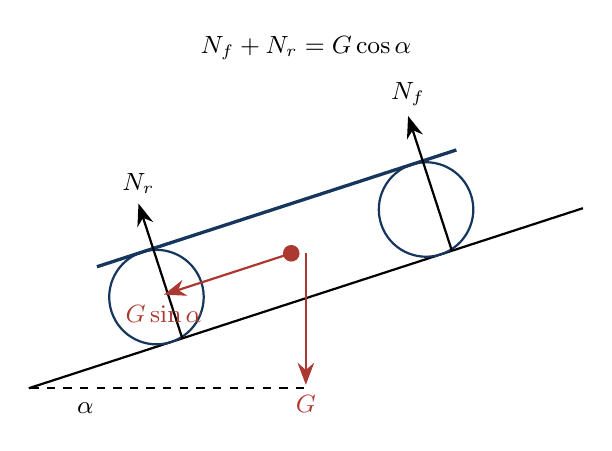
\begin{tikzpicture}

\begin{scope}[rotate=18]\draw[thick](-3.7,0)--(3.7,0);\draw[blue,thick](-1.8,.6)circle(.6);\draw[blue,thick](1.8,.6)circle(.6);\draw[very thick,blue](-2.4,1.2)--(2.4,1.2);\fill[red](0,.6)circle(3pt);\draw[arrow](-1.65,0)--(-1.65,1.8)node[above]{$N_r$};\draw[arrow](1.95,0)--(1.95,1.8)node[above]{$N_f$};\draw[arrow,red](0,.6)--(-1.7,.6)node[below]{$G\sin\alpha$};\end{scope}\draw[arrow,red](0,.57)--(0,-1.1)node[below]{$G$};\draw[dashed](-3.5,-1.14)--(0,-1.14);\node[below]at(-2.8,-1.2){$\alpha$};\node[above]at(0,2.9){$N_f+N_r=G\cos\alpha$};

\end{tikzpicture}
\begin{tikzpicture}

\node[box,fill=blue!8](a)at(0,0){偏移$\Delta/2$\\滚阻矩$kN^2/2$};\node[box](b)at(4.8,0){单轮力矩平衡\\确定$f_f,f_r$};\node[box](c)at(4.8,-2){质心力矩\\$N_r-N_f=2\tau/l$};\node[box,fill=red!8](d)at(0,-2){功率、力矩\\接地、摩擦};\draw[arrow](a)--(b);\draw[arrow](b)--(c);\draw[arrow](c)--(d);

\end{tikzpicture}
\end{document}
